\chapter{Les devis\index{Devis}}
Les devis représentent l'une des fonctionnalités principales de l'application. Il est possible de créer plusieurs devis pour un seul projet d'un client. 
\section{Liste des devis\index{Devis!Liste}}
Pour afficher la liste des devis d'un projet il faut, à partir du panneau contenant la liste des projets d'un client, faire un double clic sur le projet en question.
\begin{figure}[H]
	\centering
	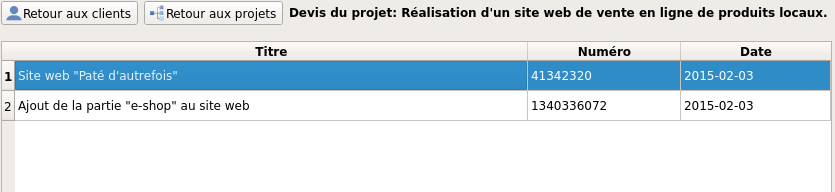
\includegraphics[width=12cm]{screens/ihmDevis.png}
	\caption{Liste des devis d'un projet}
\end{figure}

\section{Ajouter un devis\index{Devis!Ajouter}}
Pour ajouter un devis, il est nécessaire de sélectionner un client dans le panneau central (si l'on est dans la liste des projets ou des devis, le nouveau devis sera automatiquement ajouté à ce client). Une fois le client selectionné on crée un nouveau devis en cliquant sur le bouton << Nouveau devis >> de la barre d'outils ou via le menu << Client $\rightarrow$ Nouveau devis >>. 
\begin{figure}[H]
	\centering
	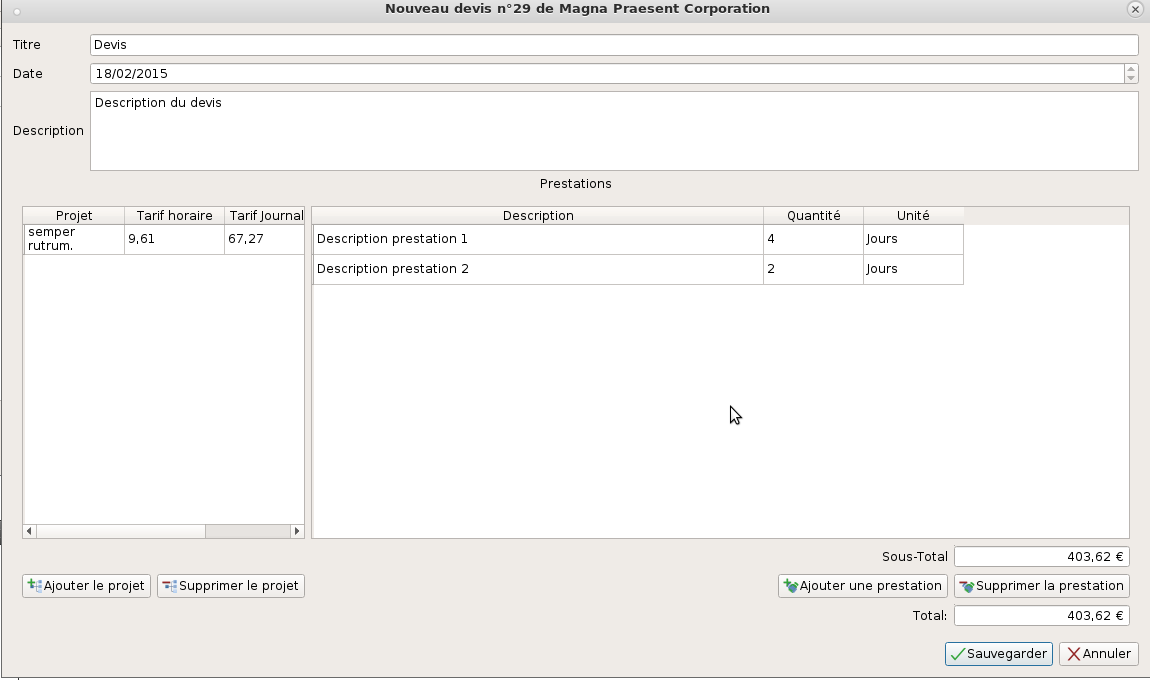
\includegraphics[width=7cm]{screens/creerDevis.png}
	\caption{Créer un nouveau devis à un projet client}
\end{figure}
Un devis possède un titre à afficher, une date (celle du jour de création du projet), une description et la liste des prestations qui lui sont associées. 
\section{Les Prestations\index{Devis!Prestation}}
La liste des prestations sont affichées dans la fenêtre d'ajout d'un devis\index{Devis!Ajouter}. Une prestation peut être ajoutée, respectivement supprimée en utilisant les boutons << Ajouter une prestation >> et << Supprimer une prestation >>. Dans le cas d'un ajout, une nouvelle ligne est ajoutée au tableau des prestations. Cette ligne indique à quel projet est associé la prestation, une description de la prestation et le nombre d'heures que l'on va y consacrer. 